\newcommand{\QpuDocTitle}{QPU Examples and Troubleshooting}
\newcommand{\QpuDocSubtitle}{Runnable Protocols, Diagnostics, and Correction Lab}
\newcommand{\QpuHeaderTitle}{Examples and Troubleshooting}
\newcommand{\QpuDocDescription}{%
Complete examples with line-by-line explanations, advanced worked circuits
(adders, comparators, parity, phase kickback, and oracles), custom gates,
common protocol failures,
diagnostic messages, truth-table checks, and guided Correction Lab recovery.
}
\documentclass[10pt,letterpaper]{article}

% Stable output supports docs:check even when translation uses a temporary directory.
\ifdefined\pdftrailerid
  \pdftrailerid{}
\fi

\usepackage[T1]{fontenc}
\usepackage[utf8]{inputenc}
\usepackage{lmodern}
\usepackage[margin=0.72in]{geometry}
\usepackage{amsmath,amssymb,mathtools}
\usepackage{booktabs,longtable,tabularx,array}
\usepackage[dvipsnames,table]{xcolor}
\usepackage{listings}
\usepackage{tikz}
\usepackage{enumitem}
\usepackage{fancyhdr}
\usepackage{microtype}
\usepackage[hidelinks]{hyperref}
\usepackage{bookmark}
\usepackage{titlesec}

\usetikzlibrary{arrows.meta,calc,positioning}

\definecolor{QpuNavy}{HTML}{0F172A}
\definecolor{QpuBlue}{HTML}{2563EB}
\definecolor{QpuCyan}{HTML}{0891B2}
\definecolor{QpuGreen}{HTML}{047857}
\definecolor{QpuAmber}{HTML}{B45309}
\definecolor{QpuRed}{HTML}{B91C1C}
\definecolor{QpuPaper}{HTML}{F8FAFC}
\definecolor{QpuLine}{HTML}{CBD5E1}
\definecolor{CodeBg}{HTML}{F1F5F9}
\definecolor{CodeComment}{HTML}{64748B}

\providecommand{\QpuDocTitle}{QPU Documentation}
\providecommand{\QpuDocSubtitle}{System Guide}
\providecommand{\QpuDocDescription}{A guide to the QPU circuit system.}
\providecommand{\QpuHeaderTitle}{QPU Documentation}

\hypersetup{
  pdftitle={\QpuDocTitle: \QpuDocSubtitle},
  pdfauthor={Bailey Forbes},
  pdfsubject={QPU protocol syntax, quantum gates, mathematics, and truth tables},
  pdfkeywords={QPU, quantum circuit, protocol, system syntax, truth table}
}

\pagestyle{fancy}
\fancyhf{}
\lhead{\textcolor{QpuNavy}{QPU Circuit Compiler}}
\rhead{\textcolor{QpuNavy}{\QpuHeaderTitle}}
\cfoot{\thepage}
\renewcommand{\headrulewidth}{0.3pt}

\titleformat{\section}{\Large\bfseries\color{QpuNavy}}{\thesection}{0.55em}{}
\titleformat{\subsection}{\large\bfseries\color{QpuBlue}}{\thesubsection}{0.5em}{}
\titleformat{\subsubsection}{\normalsize\bfseries\color{QpuCyan}}{\thesubsubsection}{0.45em}{}
\setlist{nosep,leftmargin=1.5em}
\setlength{\parindent}{0pt}
\setlength{\parskip}{4pt}
\setlength{\tabcolsep}{4pt}
\renewcommand{\arraystretch}{1.15}

\lstdefinelanguage{QPU}{
  morekeywords={
    PARAMS,MAIN-PROCESS,INCREASECYCLE,COMPILEPROCESS,FREE,SET,JOIN,SPLIT,
    CALL,DECLARECHILD,RUNCHILD,REC,TREC,RECUR,EXIT,IF,ELSE,ENDIF,RETURNVALS,ACCEPTVALS,MASTERVAL,SAVE_STATE,
    LOAD_STATE,CREATETOKEN,DELETETOKEN,X,Y,Z,H,S,T,CNOT,CCNOT,CZ,CY,
    SWAP,PHASE,RX,RY,RZ,CPHASE,MEASURE,NOT,AND,NAND,OR,XOR
  },
  sensitive=false,
  morecomment=[l]{\#},
  morecomment=[s]{/*}{*/},
  morestring=[b]"
}
\lstset{
  language=QPU,
  basicstyle=\ttfamily\small,
  keywordstyle=\bfseries\color{QpuBlue},
  commentstyle=\itshape\color{CodeComment},
  backgroundcolor=\color{CodeBg},
  frame=single,
  rulecolor=\color{QpuLine},
  framerule=0.4pt,
  xleftmargin=0.4em,
  framexleftmargin=0.35em,
  columns=fullflexible,
  keepspaces=true,
  showstringspaces=false,
  breaklines=true,
  aboveskip=5pt,
  belowskip=5pt
}

\newcommand{\code}[1]{\texttt{\detokenize{#1}}}
\newcommand{\ket}[1]{\lvert #1\rangle}
\newcommand{\bra}[1]{\langle #1\rvert}
\newcommand{\status}[1]{\textsf{\small #1}}
\newcommand{\implemented}{\textcolor{QpuGreen}{\status{lowered/executed}}}
\newcommand{\acceptedonly}{\textcolor{QpuAmber}{\status{accepted, not executed}}}
\newcommand{\internal}{\textcolor{QpuCyan}{\status{compiler-internal}}}

\newcommand{\GateSegment}[1]{%
\begin{tikzpicture}[baseline=-0.55ex,scale=.78]
  \draw[thick] (0,0)--(3.6,0);
  \node[left] at (0,0) {$\ket{q}$};
  \node[draw=QpuBlue,fill=QpuBlue!8,minimum width=.62cm,minimum height=.55cm,font=\bfseries] at (1.8,0) {#1};
\end{tikzpicture}}

\newcommand{\ControlledSegment}[1]{%
\begin{tikzpicture}[baseline=-0.55ex,scale=.78]
  \draw[thick] (0,.55)--(3.6,.55);
  \draw[thick] (0,-.55)--(3.6,-.55);
  \node[left] at (0,.55) {$\ket{c}$};
  \node[left] at (0,-.55) {$\ket{t}$};
  \fill[QpuNavy] (1.8,.55) circle (.09);
  \draw[thick] (1.8,.55)--(1.8,-.55);
  \node[draw=QpuBlue,fill=QpuBlue!8,circle,inner sep=1.7pt,font=\scriptsize\bfseries] at (1.8,-.55) {#1};
\end{tikzpicture}}

\newcommand{\DoubleControlledSegment}{%
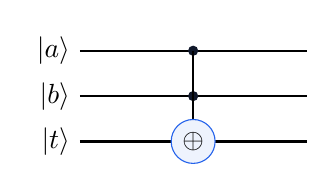
\begin{tikzpicture}[baseline=-0.55ex,scale=.72]
  \foreach \y/\n in {.8/a,0/b,-.8/t} {
    \draw[thick] (0,\y)--(4,\y);
    \node[left] at (0,\y) {$\ket{\n}$};
  }
  \fill[QpuNavy] (2,.8) circle (.09);
  \fill[QpuNavy] (2,0) circle (.09);
  \draw[thick] (2,.8)--(2,-.8);
  \node[draw=QpuBlue,fill=QpuBlue!8,circle,inner sep=2pt,font=\bfseries] at (2,-.8) {$\oplus$};
\end{tikzpicture}}

\newcommand{\SwapSegment}{%
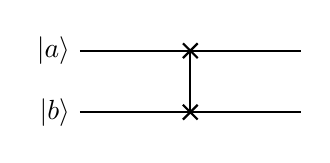
\begin{tikzpicture}[baseline=-0.55ex,scale=.78]
  \draw[thick] (0,.5)--(3.6,.5);
  \draw[thick] (0,-.5)--(3.6,-.5);
  \node[left] at (0,.5) {$\ket{a}$};
  \node[left] at (0,-.5) {$\ket{b}$};
  \draw[thick] (1.68,.38)--(1.92,.62) (1.68,.62)--(1.92,.38);
  \draw[thick] (1.68,-.38)--(1.92,-.62) (1.68,-.62)--(1.92,-.38);
  \draw[thick] (1.8,.5)--(1.8,-.5);
\end{tikzpicture}}

\newcommand{\QpuMeter}[2]{%
  \begin{scope}[shift={(#1,#2)}]
    \draw[QpuBlue,thick] (-0.28,-0.22) rectangle (0.28,0.28);
    \draw[QpuBlue,thick] (-0.18,-0.02) arc (180:0:0.18);
    \draw[QpuBlue,thick] (0,-0.02) -- (0.14,0.16);
    \fill[QpuBlue] (0,-0.02) circle (0.035);
  \end{scope}}
\newcommand{\MeasureSegment}{%
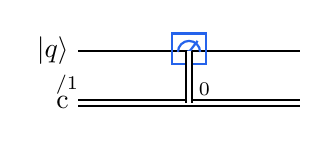
\begin{tikzpicture}[baseline=-0.55ex,scale=.78]
  \draw[thick] (0,0)--(3.6,0);
  \node[left] at (0,0) {$\ket{q}$};
  \QpuMeter{1.8}{0}
  \draw[double distance=1.4pt,thick] (0,-.85)--(3.6,-.85);
  \node[left] at (0,-.85) {c};
  \node[left,font=\scriptsize] at (0.15,-.55) {/1};
  \draw[double distance=1.4pt,thick] (1.8,0)--(1.8,-.85);
  \node[right,font=\scriptsize] at (1.8,-.62) {0};
\end{tikzpicture}}

% The hypertarget gives each gate a stable PDF named destination (gate-CNOT,
% gate-H, ...) that the workbench links to with #nameddest=.
\newcommand{\GateHeading}[3]{%
\subsection{#1 (\code{#2})}\hypertarget{gate-#2}{}
\begin{center}#3\end{center}}

% Short framed callouts. The body is boxed, so it cannot contain lstlisting
% and should stay short enough to fit on one page.
\newsavebox{\QpuCalloutBox}
\newenvironment{QpuCallout}[2]{%
  \def\QpuCalloutColor{#1}%
  \setlength{\fboxrule}{0.6pt}%
  \par\smallskip\noindent
  \begin{lrbox}{\QpuCalloutBox}%
  \begin{minipage}{\dimexpr\linewidth-2\fboxsep-2\fboxrule\relax}%
  \setlength{\parskip}{3pt}%
  {\bfseries\color{#1}#2}\par
}{%
  \end{minipage}%
  \end{lrbox}%
  \fcolorbox{\QpuCalloutColor}{\QpuCalloutColor!6}{\usebox{\QpuCalloutBox}}%
  \par\smallskip
}
\newenvironment{beginnerbox}[1][Beginner note]{\begin{QpuCallout}{QpuGreen}{#1}}{\end{QpuCallout}}
\newenvironment{trybox}[1][Try it in the Circuit builder]{\begin{QpuCallout}{QpuBlue}{#1}}{\end{QpuCallout}}
\newenvironment{cautionbox}[1][Watch out]{\begin{QpuCallout}{QpuAmber}{#1}}{\end{QpuCallout}}

% Workbench selectors on the left, the circuit diagram they produce on the
% right. #1 is the gate name shown in the Gate selector and on the target.
\newcommand{\WorkbenchControlMap}[1]{%
\begin{tikzpicture}[font=\small,>={Latex[length=2mm]}]
  \tikzset{ui/.style={draw=##1,rounded corners=2pt,anchor=west,minimum width=3.9cm,minimum height=.55cm,inner sep=3pt}}
  \node[ui=QpuLine,fill=CodeBg] at (0,1.75) {\textsf{Gate:} \textbf{#1}};
  \node[ui=QpuBlue,fill=QpuBlue!8] (a) at (0,.95) {\textsf{Control A:} \textbf{q0}};
  \node[ui=QpuBlue,fill=QpuBlue!8] (b) at (0,.15) {\textsf{Control B:} \textbf{q1}};
  \node[ui=QpuRed,fill=QpuRed!6] (t) at (0,-.65) {\textsf{Target particle:} \textbf{q2}};
  \node[font=\scriptsize\bfseries,color=QpuNavy,anchor=west] at (0,2.45) {Interactive workbench};
  \node[font=\scriptsize\bfseries,color=QpuNavy] at (7.4,2.45) {Circuit canvas};
  \foreach \y/\q in {.95/q0,.15/q1,-.65/q2} {
    \draw[thick] (5.6,\y)--(9.2,\y);
    \node[left,font=\scriptsize] at (5.6,\y) {\q};
  }
  \draw[->,dashed,QpuBlue] (a.east)--(5.05,.95);
  \draw[->,dashed,QpuBlue] (b.east)--(5.05,.15);
  \draw[->,dashed,QpuRed] (t.east)--(5.05,-.65);
  \fill[QpuNavy] (7.4,.95) circle (.09);
  \fill[QpuNavy] (7.4,.15) circle (.09);
  \draw[thick] (7.4,.95)--(7.4,-.65);
  \node[draw=QpuRed,fill=QpuRed!6,circle,inner sep=1.5pt,font=\bfseries] at (7.4,-.65) {$\oplus$};
  \node[anchor=west,font=\scriptsize] at (9.3,.95) {$A$: read, left unchanged};
  \node[anchor=west,font=\scriptsize] at (9.3,.15) {$B$: read, left unchanged};
  \node[anchor=west,font=\scriptsize] at (9.3,-.65) {$t' = t\oplus(A\land B)$: written};
\end{tikzpicture}}

\newcommand{\QpuTitlePage}{%
\begin{titlepage}
\pagecolor{QpuPaper}
\centering
\vspace*{1.15in}
{\Huge\bfseries\color{QpuNavy} \QpuDocTitle\par}
\vspace{0.2in}
{\LARGE\color{QpuBlue} \QpuDocSubtitle\par}
\vspace{0.55in}
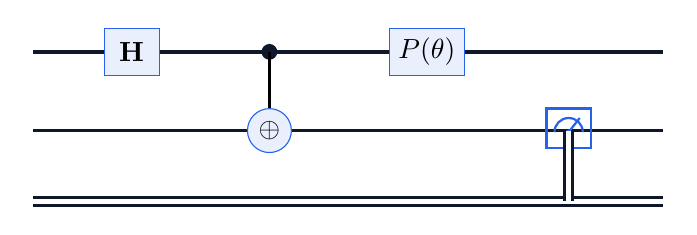
\begin{tikzpicture}
  \draw[very thick,QpuNavy] (0,1)--(8,1);
  \draw[very thick,QpuNavy] (0,0)--(8,0);
  \draw[double distance=1.6pt,very thick,QpuNavy] (0,-.9)--(8,-.9);
  \node[draw=QpuBlue,fill=QpuBlue!10,minimum width=.7cm,minimum height=.6cm,font=\bfseries] at (1.25,1) {H};
  \fill[QpuNavy] (3,1) circle (.1);
  \draw[very thick] (3,1)--(3,0);
  \node[draw=QpuBlue,fill=QpuBlue!10,circle,inner sep=2pt] at (3,0) {$\oplus$};
  \node[draw=QpuBlue,fill=QpuBlue!10,minimum width=.8cm,minimum height=.6cm,font=\bfseries] at (5,1) {$P(\theta)$};
  \QpuMeter{6.8}{0}
  \draw[double distance=1.6pt,very thick,QpuNavy] (6.8,0)--(6.8,-.9);
\end{tikzpicture}
\vfill
{\large Bailey Forbes\par}
{\large September 13, 2026\par}
\vspace{0.35in}
\begin{minipage}{0.82\textwidth}
\small\color{QpuNavy}
\QpuDocDescription
\end{minipage}
\vfill
\end{titlepage}
\nopagecolor
}

% Widen the TOC number column so two-digit subsections (13.10) keep a gap before the title.
\makeatletter
\renewcommand*\l@subsection{\@dottedtocline{2}{1.5em}{2.8em}}
\renewcommand*\l@subsubsection{\@dottedtocline{3}{4.3em}{3.6em}}
\makeatother

\newcommand{\QpuContents}{%
\pagenumbering{roman}
\tableofcontents
\clearpage
\pagenumbering{arabic}
}


\begin{document}
\QpuTitlePage
\QpuContents

\section{How to use the QPU website}

This chapter assumes no programming experience. You can build circuits by
clicking controls, or edit the text protocol directly. Both paths describe the
same circuit.

\subsection{Five programming words used in this guide}

\begin{description}
  \item[Source text] The human-readable instructions in the protocol editor.
  It is ordinary text, like a note, with one QPU instruction per logical line.
  \item[Instruction] One action for the QPU system, such as SET, H, CNOT, or
  MEASURE. The first word says what action to perform.
  \item[Argument] Extra information after an instruction. In
  \code{SET Q 0p}, Q and 0p are arguments: they say which wire and which state.
  \item[Compile] Translate source text into the ordered visual gates that the
  simulator can run. Compilation checks spelling, required inputs, and targets.
  \item[Run] Apply the compiled gates to the selected starting state. Running
  changes simulator state; it does not rewrite the source text.
\end{description}

\subsection{Interface words and how they relate}

\begin{center}
\begin{tabularx}{\textwidth}{>{\bfseries}l X}
\toprule
Word on screen or in source & Meaning\\
\midrule
Particle / qubit & One simulated quantum two-state system. The interface may
say particle where circuit theory says qubit.\\
Wire & The horizontal visual path followed by one qubit through the circuit.\\
Token & A source-text name, such as Q or Carry, that resolves to a wire.\\
Register & One or more qubit wires considered as a group.\\
Gate & A box or controlled symbol that transforms state.\\
Target & The wire changed by a gate.\\
Control & A wire whose state decides whether a controlled gate acts.\\
Protocol / process & The complete source description of a named circuit.\\
\bottomrule
\end{tabularx}
\end{center}

\subsection{Run a bundled example without writing code}

\begin{enumerate}
  \item Open the navigation menu and choose \textbf{Circuit builder}.
  \item Find \textbf{Load a starter circuit} and choose an example.
  \item Inspect the horizontal wires and gate blocks on the circuit canvas.
  \item Choose \textbf{Play Sequence} to watch gates advance, or
  \textbf{Run all} to jump to the final state.
  \item Choose \textbf{Measure all} if the circuit has not already measured
  its outputs.
  \item Read the particle/state display and runtime log. A measured qubit is a
  classical 0 or 1 outcome for that run.
  \item Choose \textbf{Reset state} before repeating the same experiment.
\end{enumerate}

\subsection{Compile a complete protocol}

Listings marked \textbf{Complete runnable protocol} may be copied as a whole:

\textbf{Complete runnable protocol}
\begin{lstlisting}
MAIN-PROCESS FirstWebsiteCircuit
CREATETOKEN -I Q
SET Q 0p
H -I Q -O Q
MEASURE -I Q
RETURNVALS Q
\end{lstlisting}

\begin{enumerate}
  \item Scroll to \textbf{Compile text into a circuit}.
  \item Replace the editor contents with the complete listing.
  \item Choose \textbf{Compile protocol}.
  \item Read \textbf{Protocol checks}. Zero errors means compilation may
  proceed. Warnings identify accepted syntax that may not behave as expected.
  \item Return to the run controls and choose \textbf{Run all}.
\end{enumerate}

\textbf{Expected result:} the H gate prepares equal 0 and 1 amplitudes.
MEASURE returns either 0 or 1. Repeating from Reset state should produce both
outcomes over many runs.

\subsection{Complete examples versus fragments}

This documentation uses three listing labels:
\begin{description}
  \item[Complete runnable protocol] Copy the entire block into the protocol
  editor and compile it.
  \item[Instruction fragment] A few lines demonstrating one syntax rule. Add
  them to a complete process rather than compiling the fragment alone.
  \item[Companion metadata] Truth-table text saved separately as
  \code{.qpuio}; do not paste it into the protocol editor.
\end{description}

\subsection{When protocol checks report a problem}

An \textbf{error} blocks successful compilation. A \textbf{warning} means the
text is accepted but may use inactive, incomplete, or surprising behavior.
Each diagnostic gives a line number, the relevant source line when available,
and a suggested correction.

Choose \textbf{Open Correction Lab for guided help} below the diagnostic list
when the correction is not obvious. The Correction Lab can test a protocol,
probe outputs, explain failures, and propose gate-level guidance. It does not
change protected bundled truth tables.

\subsection{Saving and reopening work}

Choose \textbf{Download as .qpucir} to save protocol source. The
\code{-qpucir.txt} option contains the same source for devices that only handle
plain text files. Use the navigation menu's \textbf{Upload files} page to
reopen a protocol, optionally together with its matching \code{.qpuio}
truth-table metadata.

\section{First circuit: from source to result}

The shortest useful learning path is to prepare one qubit, transform it,
measure it, and declare it as an output:

\textbf{Complete runnable protocol}
\begin{lstlisting}
MAIN-PROCESS FirstCircuit
CREATETOKEN -I Q
SET Q 0p
H -I Q -O Q
MEASURE -I Q
RETURNVALS Q
\end{lstlisting}

\subsection{Read the program line by line}

\begin{enumerate}
  \item \code{MAIN-PROCESS FirstCircuit} gives the protocol a name.
  \item \code{CREATETOKEN -I Q} reserves a logical wire named Q.
  \item \code{SET Q 0p} prepares Q in the basis state $\ket0$.
  \item \code{H -I Q -O Q} applies Hadamard to that same wire, producing
  $\ket+=(\ket0+\ket1)/\sqrt2$.
  \item \code{MEASURE -I Q} samples 0 or 1 and collapses the state.
  \item \code{RETURNVALS Q} declares Q as the first public result.
\end{enumerate}

\begin{center}
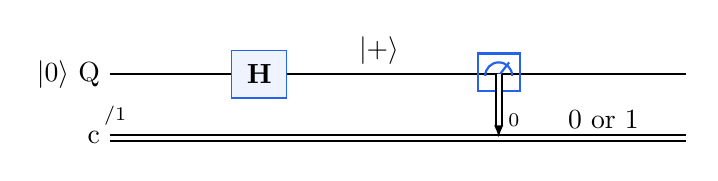
\begin{tikzpicture}[scale=.95]
  \draw[thick] (0,0)--(7.7,0);
  \draw[double distance=1.4pt,thick] (0,-.85)--(7.7,-.85);
  \node[left] at (0,0) {$\ket0$ Q};
  \node[left] at (0,-.85) {c};
  \node[left,font=\scriptsize] at (0.35,-.55) {/1};
  \node[draw=QpuBlue,fill=QpuBlue!8,minimum width=.7cm,minimum height=.6cm,font=\bfseries] at (2,0) {H};
  \node[above] at (3.6,0) {$\ket+$};
  \QpuMeter{5.2}{0}
  \draw[double distance=1.4pt,thick,-{Latex[length=1.6mm]}] (5.2,0)--(5.2,-.85);
  \node[right,font=\scriptsize] at (5.2,-.62) {0};
  \node[above] at (6.6,-.85) {0 or 1};
\end{tikzpicture}
\end{center}

\subsection{What one run means}

One execution gives one random-looking sample. For this circuit, theory predicts
equal probability for 0 and 1. Getting 0 once does not mean H failed, and
getting 1 once does not prove a bias. Repeat the circuit to compare observed
frequencies with the predicted distribution.

\subsection{Adding user-controlled input}

Move a wire into PARAMS when callers or truth-table rows should choose its
start state:

\textbf{Complete runnable protocol}
\begin{lstlisting}
PARAMS: Input:state

MAIN-PROCESS Inverter
X -I Input -O Input
MEASURE -I Input
RETURNVALS Input
\end{lstlisting}
The matching deterministic truth table is:
\begin{center}
\begin{tabular}{c|c}\toprule Input & Output\\\midrule
\code{0p}&\code{1p}\\
\code{1p}&\code{0p}\\\bottomrule
\end{tabular}
\end{center}
The rest of this manual explains every symbol in these examples before moving
to multi-qubit gates, child processes, and full truth-table files.


\section{Worked example: reversible half-adder}

A half-adder adds two one-bit numbers without a carry input. Classical theory
defines two outputs:
\[
\mathrm{Sum}=A\oplus B,\qquad
\mathrm{Carry}=A\land B.
\]
The name \emph{half-adder} means it handles half of the full-adder interface:
there is no $C_{\rm in}$ input.

\subsection{Classical specification}

\begin{center}
\begin{tabular}{cc|cc|c}
\toprule
$A$&$B$&Carry&Sum&Binary interpretation\\
\midrule
0&0&0&0&$0+0=00_2$\\
0&1&0&1&$0+1=01_2$\\
1&0&0&1&$1+0=01_2$\\
1&1&1&0&$1+1=10_2$\\
\bottomrule
\end{tabular}
\end{center}
The Carry column is the high-order bit and Sum is the low-order bit. In the
last row, decimal $1+1=2$, written $10_2$ in binary.

\subsection{QPU protocol}

\textbf{Complete runnable protocol}
\begin{lstlisting}
PARAMS: A:state B:state

MAIN-PROCESS HalfAdder
CREATETOKEN -I Carry Sum
SET Carry 0p
SET Sum 0p

XOR -I A B -O Sum
AND -I A B -O Carry

MEASURE -I Carry
MEASURE -I Sum
RETURNVALS Carry Sum
\end{lstlisting}

\subsection{What every term is doing}

\begin{enumerate}
  \item \textbf{PARAMS} declares A and B as caller-controlled state inputs.
  In a basis-state truth-table test they receive \code{0p} or \code{1p}.
  \item \textbf{Carry and Sum are workspace targets.} CREATETOKEN reserves their
  names; SET prepares both in zero.
  \item \textbf{XOR uses A and B as controls/inputs.} It mutates Sum according
  to $s'=s\oplus A\oplus B$. Because $s=0$, the result is $A\oplus B$.
  \item \textbf{AND uses the same preserved controls.} It mutates Carry
  according to $c'=c\oplus(A\land B)$. Because $c=0$, Carry becomes the
  classical carry predicate.
  \item \textbf{MEASURE produces classical samples.} For basis inputs this
  example is deterministic. If A or B is in superposition, outputs may be
  entangled with the inputs and measurement samples a branch.
  \item \textbf{RETURNVALS defines interface order.} Carry is output column
  zero and Sum is output column one. It does not perform measurement itself.
\end{enumerate}

\begin{center}
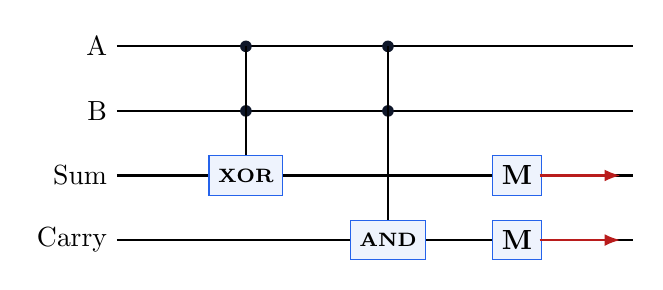
\begin{tikzpicture}[scale=.82]
  \foreach \y/\name in {1.5/A,.5/B,-.5/Sum,-1.5/Carry} {
    \draw[thick] (0,\y)--(8,\y);
    \node[left] at (0,\y) {\name};
  }
  \fill[QpuNavy] (2,1.5) circle (.09);
  \fill[QpuNavy] (2,.5) circle (.09);
  \draw[thick] (2,1.5)--(2,-.5);
  \node[draw=QpuBlue,fill=QpuBlue!8,minimum width=.72cm,minimum height=.5cm,font=\scriptsize\bfseries] at (2,-.5) {XOR};
  \fill[QpuNavy] (4.2,1.5) circle (.09);
  \fill[QpuNavy] (4.2,.5) circle (.09);
  \draw[thick] (4.2,1.5)--(4.2,-1.5);
  \node[draw=QpuBlue,fill=QpuBlue!8,minimum width=.72cm,minimum height=.5cm,font=\scriptsize\bfseries] at (4.2,-1.5) {AND};
  \node[draw=QpuBlue,fill=QpuBlue!8,minimum width=.6cm,minimum height=.5cm,font=\bfseries] at (6.2,-.5) {M};
  \node[draw=QpuBlue,fill=QpuBlue!8,minimum width=.6cm,minimum height=.5cm,font=\bfseries] at (6.2,-1.5) {M};
  \draw[-{Latex[length=2mm]},QpuRed,thick] (6.55,-.5)--(7.8,-.5);
  \draw[-{Latex[length=2mm]},QpuRed,thick] (6.55,-1.5)--(7.8,-1.5);
\end{tikzpicture}
\end{center}

\begin{beginnerbox}[Which wires change?]
Only the two outputs. A and B are \emph{read} by both gates and come out
exactly as they went in. Sum and Carry are \emph{workspace}: they start at 0
and each receives one answer. Keeping the inputs is what makes the circuit
reversible, and it is why a quantum half-adder needs four wires where a
classical one draws two inputs and two outputs.
\end{beginnerbox}

\subsection{Build the Carry gate in the workbench}

The AND line of the protocol corresponds to these workbench choices. With A
on q0, B on q1, and Carry on q2:
\begin{center}
\WorkbenchControlMap{AND}
\end{center}
\begin{trybox}
Choose the \emph{Half adder} starter circuit. Set \textbf{q0 start} and
\textbf{q1 start} to each combination of \code{0p} and \code{1p}, choose
\textbf{Run all} each time, and check the measured Sum and Carry against the
table above.
\end{trybox}

\subsection{Reversible state equation}

Before measurement, the full basis-state action is
\[
\ket{A,B,s,c}\longmapsto
\ket{A,B,s\oplus A\oplus B,\ c\oplus(A\land B)}.
\]
The familiar half-adder is the special case $s=c=0$. Writing the complete
equation avoids a common mistake: XOR and AND do not overwrite arbitrary
targets. They reversibly combine results with the targets' previous states.

\subsection{Companion truth-table metadata}

\begin{lstlisting}
MAIN-PROCESS: HalfAdder
INPUTS: A B
OUTPUTS: Carry Sum
# A B Carry Sum
0 0p 0p 0p 0p
1 0p 1p 0p 1p
2 1p 0p 0p 1p
3 1p 1p 1p 0p
\end{lstlisting}
This file compares the measured QPU outputs with the classical half-adder
specification. Passing all four rows demonstrates basis-state equivalence; it
does not by itself characterize phases for superposition inputs.


\section{Worked example: randomness versus interference}

Classical random choice and quantum superposition can produce identical
single-measurement frequencies. They are not the same theory. This example
uses an intermediate phase change to distinguish them.

\subsection{Classical fair coin model}

Imagine a classical variable R chosen by a fair coin:
\[
P(R=0)=\frac12,\qquad P(R=1)=\frac12.
\]
Once chosen, R is one definite value even if the observer has not looked.
Applying classical NOT changes 0 to 1 and 1 to 0, but the distribution remains
half and half. There is no operation that makes the probability of one hidden
branch cancel the other branch.

\subsection{Quantum preparation with Hadamard}

\begin{lstlisting}
MAIN-PROCESS QuantumCoin
CREATETOKEN -I Q
SET Q 0p
H -I Q -O Q
MEASURE -I Q
RETURNVALS Q
\end{lstlisting}
Before measurement,
\[
\ket0\xrightarrow{H}
\ket+=\frac{\ket0+\ket1}{\sqrt2}.
\]
The amplitudes are $1/\sqrt2$ and $1/\sqrt2$; squaring magnitudes gives the
same half-and-half distribution as the classical coin. If measurement happens
now, this experiment alone cannot distinguish the two descriptions.

\subsection{Insert phase and recombine paths}

\begin{lstlisting}
MAIN-PROCESS PhaseInterference
CREATETOKEN -I Q
SET Q 0p
H -I Q -O Q
Z -I Q -O Q
H -I Q -O Q
MEASURE -I Q
RETURNVALS Q
\end{lstlisting}
Track the state:
\[
\ket0
\xrightarrow{H}
\frac{\ket0+\ket1}{\sqrt2}
\xrightarrow{Z}
\frac{\ket0-\ket1}{\sqrt2}
\xrightarrow{H}
\ket1.
\]

\subsection{Term-by-term explanation}

\begin{description}
  \item[Superposition] After the first H, both basis states have coherent
  amplitudes. No measurement has selected one.
  \item[Phase] Z multiplies only the $\ket1$ amplitude by $-1=e^{i\pi}$. Its
  magnitude remains $1/\sqrt2$, so immediate 0/1 probabilities remain equal.
  \item[Relative phase] The plus relationship between amplitudes becomes a
  minus relationship. A global minus on both terms would not matter; changing
  only one term does.
  \item[Interference] The final H mixes the basis amplitudes. Contributions to
  the $\ket0$ output cancel, while contributions to $\ket1$ add.
  \item[Measurement] The final state is $\ket1$, so measurement returns 1 with
  probability one.
\end{description}

The cancellation can be seen directly from matrix multiplication:
\[
H\frac1{\sqrt2}
\begin{bmatrix}1\\-1\end{bmatrix}
=
\frac12
\begin{bmatrix}1&1\\1&-1\end{bmatrix}
\begin{bmatrix}1\\-1\end{bmatrix}
=
\frac12\begin{bmatrix}0\\2\end{bmatrix}
=\begin{bmatrix}0\\1\end{bmatrix}.
\]
Classical probability weights are nonnegative and would add rather than cancel.
Quantum amplitudes are signed or complex, so phase can create destructive and
constructive interference before the Born rule turns amplitudes into
probabilities.

\subsection{Comparison table}

\begin{center}
\begin{tabularx}{\textwidth}{>{\bfseries}lXX}
\toprule
Question & Classical fair coin & H--Z--H quantum circuit\\
\midrule
State before observation & One hidden definite bit sampled fairly &
Coherent complex amplitude vector\\
Effect of middle sign/phase & No probability analogue that preserves a fair
distribution and later cancels a branch & Z changes relative phase without
changing immediate basis probabilities\\
Can paths cancel? & No; probabilities add & Yes; amplitudes add and may cancel\\
Final result in this example & Still a distribution unless another classical
rule forces a value & Deterministic 1\\
\bottomrule
\end{tabularx}
\end{center}


\section{Advanced worked circuits}
\hypertarget{advanced-circuits}{}

The earlier examples use one or two gates. The circuits in this chapter show
that the same pieces scale to arithmetic, comparison, parity, phase tricks,
and small oracle algorithms. Every listing is a \textbf{Complete runnable
protocol}: paste it into \textbf{Compile text into a circuit}, choose
\textbf{Compile protocol}, then \textbf{Run all}. Circuits with \code{PARAMS}
can also be checked row by row in the \textbf{Circuit correction lab} with
\textbf{Infer truth table}, \textbf{Probe outputs}, and \textbf{Test circuit}.

\begin{beginnerbox}[One pattern runs through this whole chapter]
Inputs are \emph{read}, never overwritten. Each answer is written into a
fresh output wire that starts at 0, using the rule
$\text{target}' = \text{target}\oplus f(\text{inputs})$. When a circuit needs a
temporary helper wire, it computes the helper, uses it, and then runs the same
gates again to return the helper to 0 (\emph{uncomputation}).
\end{beginnerbox}

\subsection{Full adder from primitive gates}

A full adder adds three bits $A$, $B$, and a carry-in $C_{\rm in}$:
\[
\mathrm{Sum}=A\oplus B\oplus C_{\rm in},\qquad
C_{\rm out}=\operatorname{majority}(A,B,C_{\rm in})
=(A\land B)\oplus(A\land C_{\rm in})\oplus(B\land C_{\rm in}).
\]

\textbf{Complete runnable protocol}
\begin{lstlisting}
PARAMS: A:state B:state Cin:state

MAIN-PROCESS FlatFullAdder
CREATETOKEN -I Cout Sum
SET Cout 0p
SET Sum 0p

# Stage 1: Sum collects the parity of the three inputs.
CNOT -I A -O Sum
CNOT -I B -O Sum
CNOT -I Cin -O Sum

# Stage 2: Cout flips once for every pair of inputs that are both 1.
CCNOT -I A B -O Cout
CCNOT -I A Cin -O Cout
CCNOT -I B Cin -O Cout

MEASURE -I Cout
MEASURE -I Sum
RETURNVALS Cout Sum
\end{lstlisting}

\textbf{Why the carry works:} if exactly two inputs are 1, one pair is active
and Cout flips once, to 1. If all three are 1, all three pairs are active and
Cout flips three times, which still leaves 1. With zero or one active input no
pair fires. That is exactly ``at least two of three'', the majority function.
The bundled \code{SingleBitFullAdder} is the same circuit.

\subsection{Two-bit adder built from a child process}

Multi-bit addition chains full adders: the carry out of bit 0 becomes the
carry in of bit 1. \code{RUNCHILD} reuses the bundled \code{SingleBitFullAdder}
for each bit, so the parent only describes the wiring.

\textbf{Complete runnable protocol}
\begin{lstlisting}
PARAMS: A1:state A0:state B1:state B0:state

MAIN-PROCESS TwoBitRippleAdder
DECLARECHILD SingleBitFullAdder
CREATETOKEN -I NoCarry C0 S0 C1 S1
SET NoCarry 0p

# Bit 0: A0 + B0 with no incoming carry.
RUNCHILD SingleBitFullAdder -I A0 B0 NoCarry -O C0 S0
# Bit 1: A1 + B1 plus the carry from bit 0.
RUNCHILD SingleBitFullAdder -I A1 B1 C0 -O C1 S1

MEASURE -I C1
MEASURE -I S1
MEASURE -I S0
RETURNVALS C1 S1 S0
\end{lstlisting}

The outputs read as a three-bit binary number $C_1S_1S_0$. For example,
$A=11_2=3$ and $B=10_2=2$ give $C_1S_1S_0=101_2=5$. The bundled
\code{TwoBitFullAdder} and \code{FourBitFullAdder} extend the same chain with
an explicit carry input and more bits.

\subsection{Reversible comparator: is A greater than B?}

For single bits, $A>B$ exactly when $A=1$ and $B=0$, that is
$A\land\neg B$. The circuit negates B temporarily, uses it, and restores it.

\textbf{Complete runnable protocol}
\begin{lstlisting}
PARAMS: A:state B:state

MAIN-PROCESS GreaterThan
CREATETOKEN -I Gt
SET Gt 0p

X -I B -O B
AND -I A B -O Gt
X -I B -O B

MEASURE -I Gt
RETURNVALS Gt
\end{lstlisting}
\begin{center}
\begin{tabular}{cc|c}\toprule $A$&$B$&Gt\\\midrule
0&0&0\\0&1&0\\1&0&1\\1&1&0\\\bottomrule\end{tabular}
\end{center}
The second X is what keeps the circuit honest: without it, B would leave the
circuit inverted and any later gate reading B would see the wrong value.

\subsection{Two-bit equality with uncomputation}

Two numbers are equal when every bit agrees. This circuit writes a
``this bit differs'' flag for each bit, combines the flags, and then cleans the
flags up.

\textbf{Complete runnable protocol}
\begin{lstlisting}
PARAMS: A1:state A0:state B1:state B0:state

MAIN-PROCESS TwoBitEquality
CREATETOKEN -I D1 D0 Eq
SET D1 0p
SET D0 0p
SET Eq 1p

# Compute: D = 1 where the bits differ.
XOR -I A1 B1 -O D1
XOR -I A0 B0 -O D0

# Eq starts at 1 and flips if any bit differs.
OR -I D1 D0 -O Eq

# Uncompute: the same XORs return D1 and D0 to 0.
XOR -I A1 B1 -O D1
XOR -I A0 B0 -O D0

MEASURE -I Eq
MEASURE -I D1
MEASURE -I D0
RETURNVALS Eq D1 D0
\end{lstlisting}

Three ideas meet here:
\begin{description}
  \item[A target that starts at 1] \code{SET Eq 1p} makes
  $\mathrm{Eq}'=1\oplus(D_1\lor D_0)=\neg(D_1\lor D_0)$. Starting a target
  at 1 turns ``flip when true'' into ``clear when true''.
  \item[Uncomputation] XOR is its own inverse, so repeating the two XOR lines
  returns $D_1$ and $D_0$ to 0 for every input.
  \item[Proof by truth table] Returning D1 and D0 lets a truth-table test
  confirm the cleanup. In all 16 rows those two columns must be 0.
\end{description}

\subsection{Parity of four bits}

Parity is 1 when an odd number of inputs are 1. Each CNOT adds one input into
the target modulo 2.

\textbf{Complete runnable protocol}
\begin{lstlisting}
PARAMS: A:state B:state C:state D:state

MAIN-PROCESS FourBitParity
CREATETOKEN -I P
SET P 0p

CNOT -I A -O P
CNOT -I B -O P
CNOT -I C -O P
CNOT -I D -O P

MEASURE -I P
RETURNVALS P
\end{lstlisting}
Parity checks are how error-detecting codes notice a single flipped bit. The
two-input \code{XOR -I A B -O P} is shorthand for the first two CNOT lines.

\subsection{Phase kickback}
\hypertarget{phase-kickback}{}

A CNOT never changes its control's 0/1 value, but it \emph{can} change the
control's phase. Put the target in $\ket-=(\ket0-\ket1)/\sqrt2$: flipping
$\ket-$ gives $-\ket-$, so ``flip the target'' becomes ``multiply by $-1$'',
and that sign attaches to the control's $\ket1$ branch.

\textbf{Complete runnable protocol}
\begin{lstlisting}
MAIN-PROCESS PhaseKickback
CREATETOKEN -I Ctrl Tgt
SET Ctrl 0p
SET Tgt 1p

H -I Ctrl -O Ctrl
H -I Tgt -O Tgt
CNOT -I Ctrl -O Tgt
H -I Ctrl -O Ctrl

MEASURE -I Ctrl
RETURNVALS Ctrl
\end{lstlisting}
\[
\ket{+}\ket{-}\xrightarrow{\mathrm{CNOT}}\ket{-}\ket{-}
\xrightarrow{H\text{ on Ctrl}}\ket{1}\ket{-}.
\]
Ctrl measures 1 every time. Change \code{SET Tgt 1p} to \code{SET Tgt 0p}
and it measures 0 every time: the target's state decided the control's
result, even though the control was never ``written''. The \emph{Phase
kickback} starter circuit shows the same effect on the canvas.

\subsection{A small oracle: finding a hidden bit string}

An \emph{oracle} is a circuit treated as a black box that computes some
$f(x)$. Here $f(x)=s\cdot x \bmod 2$ for a hidden three-bit string $s$
(Bernstein--Vazirani). Classically, finding $s$ takes three queries. Using
kickback, one query is enough.

\textbf{Complete runnable protocol}
\begin{lstlisting}
MAIN-PROCESS HiddenString101
CREATETOKEN -I In2 In1 In0 Anc
SET In2 0p
SET In1 0p
SET In0 0p
SET Anc 1p

H -I In2 -O In2
H -I In1 -O In1
H -I In0 -O In0
H -I Anc -O Anc

# Oracle for s = 101: one CNOT for every 1 in s.
CNOT -I In2 -O Anc
CNOT -I In0 -O Anc

H -I In2 -O In2
H -I In1 -O In1
H -I In0 -O In0

MEASURE -I In2
MEASURE -I In1
MEASURE -I In0
RETURNVALS In2 In1 In0
\end{lstlisting}
The measured outputs are $1,0,1$: the hidden string itself. Each oracle
CNOT kicks a phase back onto one input wire, and the final H gates turn
those phases into 0/1 values. Change which inputs have an oracle CNOT and the
answer changes to match. With a single input wire this is Deutsch's
algorithm.

\subsection{Two-qubit Grover search}

Grover's algorithm finds a marked input by boosting its amplitude. With two
qubits, one round finds the answer with certainty.

\textbf{Complete runnable protocol}
\begin{lstlisting}
MAIN-PROCESS GroverFind11
CREATETOKEN -I A B
SET A 0p
SET B 0p

# Equal superposition of 00, 01, 10, 11.
H -I A -O A
H -I B -O B

# Oracle: mark 11 with a minus sign.
CZ -I A -O B

# Diffusion: reflect every amplitude about the average.
H -I A -O A
H -I B -O B
X -I A -O A
X -I B -O B
CZ -I A -O B
X -I A -O A
X -I B -O B
H -I A -O A
H -I B -O B

MEASURE -I A
MEASURE -I B
RETURNVALS A B
\end{lstlisting}
\begin{center}
\begin{tabular}{l|cccc}\toprule
Amplitude of & $\ket{00}$ & $\ket{01}$ & $\ket{10}$ & $\ket{11}$\\\midrule
After H, H & $\tfrac12$ & $\tfrac12$ & $\tfrac12$ & $\tfrac12$\\
After oracle & $\tfrac12$ & $\tfrac12$ & $\tfrac12$ & $-\tfrac12$\\
After diffusion & 0 & 0 & 0 & $\pm1$\\\bottomrule
\end{tabular}
\end{center}
The oracle does not change any probability, since every entry still has
magnitude $\tfrac12$. The diffusion stage turns the marked sign into certainty.
Open \textbf{Outcome truth table / probabilities} on the
\textbf{Particle visualization} page after each \textbf{Step gate} to watch
the amplitudes move.

\section{Process composition and return values}

\subsection{\code{MAIN-PROCESS} (\implemented)}

\begin{lstlisting}
MAIN-PROCESS FullAdder
\end{lstlisting}
This marks the process body and supplies its catalog/library name. Compilation
already begins from the named process, so the row itself emits no gate.
The name is the first positional word after \code{MAIN-PROCESS}; avoid spaces
inside it. This name connects a protocol to catalog entries, child calls,
downloads, and companion truth-table metadata. If no marker exists, the system
uses \code{InlineProcess}, but named processes are strongly recommended.

\subsection{\code{DECLARECHILD} (\acceptedonly)}

\begin{lstlisting}
DECLARECHILD SingleBitFullAdder
\end{lstlisting}
The declaration is logged. It does not load inline source. Child bodies must
exist in the external \code{librarySources} catalog when called.
DECLARECHILD is therefore documentation/compatibility syntax rather than an
import statement. A successful declaration does not guarantee that a later
call can resolve. The process catalog supplied to compilation remains the
source of truth.

\subsection{\code{RUNCHILD} --- expand a child process (\implemented)}

\begin{lstlisting}
RUNCHILD SingleBitFullAdder \
  -I A B Cin \
  -O Carry Sum
\end{lstlisting}
The first positional argument is the child process name. Inputs bind by the
child's PARAMS order: A maps to the first parameter, B to the second, and Cin
to the third in this example. Outputs bind by the child's RETURNVALS order.
Before expansion, each bound parent output is zero-prepared once. Child-local
names receive a unique scope.

RUNCHILD is compile-time composition, not a dynamic subroutine call in a
running quantum machine. The child body is recursively expanded into the
parent's flat gate sequence. This allows the renderer and simulator to inspect
every resulting gate.

\subsection{\code{CALL} --- alternate child invocation (\implemented)}

\begin{lstlisting}
CALL SingleBitFullAdder -I A B Cin -O Carry Sum
\end{lstlisting}
CALL currently follows the same child lookup, parameter binding, output
preparation, and expansion path as RUNCHILD. RUNCHILD is used by the bundled
multi-bit protocols and makes compile-time expansion explicit; CALL is retained
as an equivalent system spelling. Both fail when the named child is absent from
the supplied process library.

\subsection{\code{RETURNVALS} (\implemented)}

\begin{lstlisting}
RETURNVALS Carry Sum
\end{lstlisting}
Positional tokens define the process's ordered public outputs. They determine
child output binding, truth-table output columns, and the UI's preferred
logical width. Do not use \code{-I} or \code{-O} here: flags would be retained
as positional return tokens.

RETURNVALS does not measure automatically. Add MEASURE instructions when
classical outcomes are required. Returning an unmeasured wire preserves it as
part of the projected quantum output shown by the system.

\subsection{\code{ACCEPTVALS} (\implemented)}

\begin{lstlisting}
CALL Child -I A B
ACCEPTVALS LocalCarry LocalSum
\end{lstlisting}
Each positional local token aliases the corresponding value from the most
recent child return list. Direct \code{-O} binding on RUNCHILD/CALL is clearer
when output names are known.

Ordering is again essential: the first ACCEPTVALS name receives the first
returned reference, and so on. The instruction refers to the most recently
completed child expansion in compiler state; inserting another child call
changes which return list is accepted.

\subsection{Nested full-adder example}

\begin{lstlisting}
# child.qpucir
PARAMS: A:state B:state Cin:state
MAIN-PROCESS ChildAdder
CREATETOKEN -I Carry Sum
SET Carry 0p
SET Sum 0p
XOR   -I A B   -O Sum
CNOT -I Cin   -O Sum
CCNOT -I A B   -O Carry
CCNOT -I A Cin -O Carry
CCNOT -I B Cin -O Carry
RETURNVALS Carry Sum
\end{lstlisting}

\begin{lstlisting}
# parent.qpucir
PARAMS: A:state B:state Cin:state
MAIN-PROCESS Parent
CREATETOKEN -I Cout Result
RUNCHILD ChildAdder -I A B Cin -O Cout Result
MEASURE -I Cout
MEASURE -I Result
RETURNVALS Cout Result
\end{lstlisting}

For basis inputs, the full-adder equations are
\[
\mathrm{Sum}=A\oplus B\oplus C_{\mathrm{in}},\qquad
C_{\mathrm{out}}=(A\land B)\oplus(A\land C_{\mathrm{in}})
\oplus(B\land C_{\mathrm{in}}).
\]
\begin{center}
\begin{tabular}{ccc|cc}\toprule
$A$&$B$&$C_{\rm in}$&$C_{\rm out}$&Sum\\\midrule
0&0&0&0&0\\0&0&1&0&1\\0&1&0&0&1\\0&1&1&1&0\\
1&0&0&0&1\\1&0&1&1&0\\1&1&0&1&0\\1&1&1&1&1\\\bottomrule
\end{tabular}
\end{center}


\section{Custom gates: packaging a circuit as one block}
\hypertarget{custom-gates}{}

A custom gate is a whole QPU process saved under a short name so that it can
be placed like any built-in block. It adds no new physics: when it runs, the
simulator replays the process's own gates, one by one, on the wires you
chose. Understanding a custom gate therefore means understanding the smaller
gates inside it.

\subsection{Register one in four steps}

\begin{enumerate}
  \item Paste the process below into the protocol editor in
  \textbf{Compile text into a circuit} and choose \textbf{Compile protocol}
  to confirm it has no errors.
  \item In \textbf{Register custom gates from QPU processes}, type
  \code{NOR} in \textbf{Gate id (palette label)} and leave
  \textbf{Source process} on \emph{Current protocol editor}.
  \item Choose \textbf{Register custom gate}. A \textbf{NOR} block appears
  under \textbf{Custom gates} in the palette and in the workbench
  \textbf{Gate} list.
  \item Place it with \textbf{Control A}, \textbf{Control B}, and
  \textbf{Target particle}, exactly like AND.
\end{enumerate}

\textbf{Complete runnable protocol}
\begin{lstlisting}
PARAMS: A:state B:state

MAIN-PROCESS NorGate
CREATETOKEN -I Out

OR -I A B -O Out
X -I Out -O Out

RETURNVALS Out
\end{lstlisting}

\subsection{How the process maps onto wires}

\begin{center}
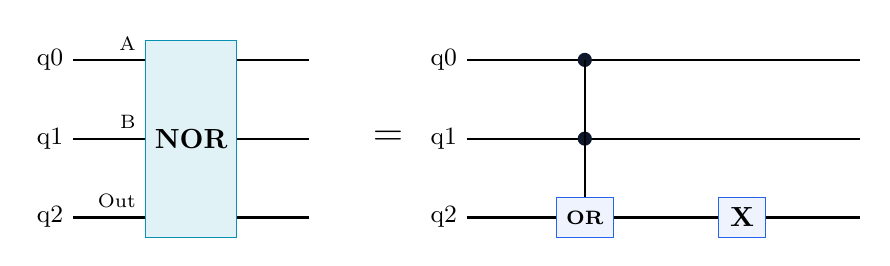
\begin{tikzpicture}[font=\small]
  \foreach \y/\q in {1/q0,0/q1,-1/q2} {
    \draw[thick] (0,\y)--(3,\y);
    \node[left] at (0,\y) {\q};
    \draw[thick] (5,\y)--(10,\y);
    \node[left] at (5,\y) {\q};
  }
  \node[draw=QpuCyan,fill=QpuCyan!12,minimum width=1.1cm,minimum height=2.5cm,font=\bfseries] at (1.5,0) {NOR};
  \node[font=\scriptsize,anchor=south east] at (0.92,1) {A};
  \node[font=\scriptsize,anchor=south east] at (0.92,0) {B};
  \node[font=\scriptsize,anchor=south east] at (0.92,-1) {Out};
  \node at (4,0) {\Large$=$};
  \fill[QpuNavy] (6.5,1) circle (.09);
  \fill[QpuNavy] (6.5,0) circle (.09);
  \draw[thick] (6.5,1)--(6.5,-1);
  \node[draw=QpuBlue,fill=QpuBlue!8,minimum width=.72cm,minimum height=.5cm,font=\scriptsize\bfseries] at (6.5,-1) {OR};
  \node[draw=QpuBlue,fill=QpuBlue!8,minimum width=.6cm,minimum height=.5cm,font=\bfseries] at (8.5,-1) {X};
\end{tikzpicture}
\end{center}

\begin{center}
\begin{tabularx}{\textwidth}{>{\bfseries}p{0.27\textwidth}X}
\toprule
In the process & Becomes, when the block is placed\\
\midrule
1st \code{PARAMS} entry & \textbf{Control A} (the lowest free wire when
dropped on the canvas).\\
2nd \code{PARAMS} entry & \textbf{Control B}. Further entries take the next
free wires.\\
1st \code{RETURNVALS} entry & \textbf{Target particle}: the only wire the
block should change.\\
Any other token & A fresh extra workspace wire that the block allocates for
itself.\\
\bottomrule
\end{tabularx}
\end{center}

The palette gives every custom block exactly one target wire, so register
processes with a single \code{RETURNVALS} output. A process with two outputs,
such as a half-adder, compiles on its own but cannot be placed as a block; use
it through \code{RUNCHILD} instead.

\subsection{Reasoning about reversibility}

A sequence of reversible gates is reversible: undo the last gate first, then
the one before it, and so on.
\[
(U_k\cdots U_2U_1)^{-1}=U_1^{-1}U_2^{-1}\cdots U_k^{-1}.
\]
NorGate is OR followed by X. Both undo themselves, so NOR undoes itself too:
placing the block twice in a row returns every wire to where it started.
Written as a rule, the block performs
\[
\mathrm{Out}'=\mathrm{Out}\oplus\neg(A\lor B),
\]
the same ``target XOR function'' shape as AND. That shape is always
reversible, because applying it again XORs the same value back out.

\begin{cautionbox}[Three things that make a custom gate irreversible]
\begin{description}
  \item[MEASURE inside the process] The block collapses its wires every time
  it runs.
  \item[SET on the output] \code{SET Out 0p} makes the compiler insert a
  hidden RESET, so the block \emph{overwrites} the target
  ($\mathrm{Out}'=f(A,B)$) instead of XORing into it. Whatever the target held
  before is erased. NorGate deliberately has no SET: a freshly compiled wire
  already starts at 0, so it passes the same truth table.
  \item[Temporary wires left dirty] Helper tokens become hidden workspace
  wires. If a helper is not returned to 0 (uncomputed), it stays entangled
  with the inputs, and the visible wires alone no longer behave reversibly.
\end{description}
\end{cautionbox}

\begin{beginnerbox}[A quick test you can run in the builder]
Place your block twice on the same wires and choose \textbf{Run all}. For a
reversible out-of-place gate, every wire ends exactly as it started. Try it
with the target's \emph{name} start set to \code{0p} and then \code{1p}. If
the target does not return, look for one of the three problems above.
\end{beginnerbox}

\subsection{Rules to remember}
\begin{itemize}
  \item The gate id must start with a letter, use only letters, digits, and
  underscores, and cannot match a built-in gate such as \code{AND}.
  \item Custom gates are saved for the current browser session only, not in
  the bundled catalog. Keep the \code{.qpucir} file to recreate one later.
  \item A custom gate can wrap a process that itself uses \code{RUNCHILD};
  the child processes are captured when you register it.
\end{itemize}

\section{Truth-table companion syntax}

Truth tables are metadata paired to a process; they are not \code{.qpucir}
commands. A protocol describes \emph{how} a circuit works; its companion
\code{.qpuio} describes selected input/output expectations.

\subsection{Text \code{.qpuio} structure}

A text table may use spaces or commas:

\begin{lstlisting}
MAIN-PROCESS: HalfAdder
INPUTS: A B
OUTPUTS: Carry Sum
# A B Carry Sum
0 0p 0p 0p 0p
1 0p 1p 0p 1p
2 1p 0p 0p 1p
3 1p 1p 1p 0p
\end{lstlisting}

\subsection{\code{MAIN-PROCESS:} table header}

The colon is required in the table format:
\begin{lstlisting}
MAIN-PROCESS: HalfAdder
\end{lstlisting}
This name associates metadata with its protocol. Notice the deliberate syntax
difference: protocol source writes \code{MAIN-PROCESS HalfAdder}, while the
truth-table header writes \code{MAIN-PROCESS: HalfAdder}.

\subsection{\code{INPUTS:} and \code{OUTPUTS:} column groups}

\begin{lstlisting}
INPUTS: A B
OUTPUTS: Carry Sum
\end{lstlisting}
These lines divide the columns into values supplied before simulation and
values checked after simulation. Their order must match the later column header.
INPUTS should correspond to state-typed PARAMS; OUTPUTS should correspond to
RETURNVALS. OUTPUTS must contain at least one name.

Explicit groups remove ambiguity. If they are absent, the loader can derive the
split only when a matching protocol is available and the combined PARAMS and
RETURNVALS widths match the table header.

\subsection{Column header row}

\begin{lstlisting}
# A B Carry Sum
\end{lstlisting}
The first nonmetadata row beginning with a hash and whitespace or comma is the
ordered column header. Here A and B are inputs, followed by Carry and Sum
outputs. Unlike an ordinary protocol hash comment, this row has structural
meaning inside a \code{.qpuio} file.

\subsection{Indexed data rows}

\begin{lstlisting}
0 0p 0p 0p 0p
1 0p 1p 0p 1p
\end{lstlisting}
The first cell is a decimal row index. Indices begin at zero and increase by
one without gaps. Remaining cells align left-to-right with the column header.
Every row must have exactly the expected width, and every state cell must be
\code{0p}, \code{1p}, or \code{sp}.

For $n$ binary input columns, a complete table contains $2^n$ rows. The usual
ordering interprets input columns most-significant first: for two inputs the
sequence is 00, 01, 10, 11. The loader checks sequential row indices, while
semantic validation also rejects duplicate input patterns.

\subsection{CSV spelling}

Commas may replace whitespace consistently:
\begin{lstlisting}
MAIN-PROCESS: HalfAdder
INPUTS: A,B
OUTPUTS: Carry,Sum
#,A,B,Carry,Sum
0,0p,0p,0p,0p
\end{lstlisting}
Spaces around commas are trimmed. Do not mix extra prose into a data row;
trailing hash comments are allowed only where the table loader can strip them
after the data content.

\subsection{Partial truth tables}

A partial table lists selected cases rather than all $2^n$ combinations. It
must contain at least one row, no duplicate input pattern, and no more than
$2^n$ rows. Partial tables are useful for state-machine transitions or focused
regressions, but passing one proves behavior only for the listed cases.

\begin{center}
\begin{tabular}{c|c|c}\toprule
Input count $n$ & Complete row count $2^n$ & Example\\\midrule
0&1&constant-output process\\
1&2&0, 1\\
2&4&00, 01, 10, 11\\
3&8&000 through 111\\
4&16&0000 through 1111\\\bottomrule
\end{tabular}
\end{center}

\subsection{JSON \code{.qpuio} envelope}

The equivalent machine-oriented JSON form is:
\begin{lstlisting}[language={}]
{
  "format": "qpuio",
  "version": 1,
  "processName": "HalfAdder",
  "inputColumns": ["A", "B"],
  "outputColumns": ["Carry", "Sum"],
  "rows": [
    ["0p", "0p", "0p", "0p"],
    ["0p", "1p", "0p", "1p"],
    ["1p", "0p", "0p", "1p"],
    ["1p", "1p", "1p", "0p"]
  ]
}
\end{lstlisting}

The \code{format} value must be \code{qpuio} and \code{version} must be 1.
Column names must be nonempty strings, outputColumns must not be empty, and
every nested row array must have exactly
\[
\text{inputColumns.length}+\text{outputColumns.length}
\]
valid cells.

\subsection{How a table test runs}

For each listed row, the runner:
\begin{enumerate}
  \item maps input cells to state PARAMS by column name and order;
  \item creates the circuit's start-state vector;
  \item executes every compiled gate, including child expansions;
  \item measures the declared RETURNVALS;
  \item compares only those measured outputs with expected output cells.
\end{enumerate}
An expected output \code{sp} accepts either measured bit. An input \code{sp}
initializes an equal plus-state superposition. Because one probabilistic sample
cannot establish a full distribution, tables are strongest for deterministic
basis-state behavior.

\subsection{Protected bundled tables}

The bundled SingleBitFullAdder, TwoBitFullAdder, FourBitFullAdder, and PhaseDemo
tables are canonical site assets. Do not rewrite them to make an experiment
pass. Create a new uploaded or corrected process/table pair when testing
different expectations. This keeps examples reproducible and prevents a
protocol correction from silently changing its specification.


\section{Complete worked protocol}

\begin{lstlisting}
PARAMS: A:state B:state Theta:float

MAIN-PROCESS BellAndLogic
CREATETOKEN -I Q0 Q1 AndOut

SET Q0 $A
SET Q1 $B
SET AndOut 0p

# Quantum segment
H -I Q0 -O Q0
CNOT -I Q0 -O Q1
PHASE=pi/4 -I Q1 -O Q1

# Basis-state comparison output
AND -I A B -O AndOut

MEASURE -I Q0
MEASURE -I Q1
MEASURE -I AndOut
RETURNVALS Q0 Q1 AndOut
\end{lstlisting}

Starting from $\ket{00}$, the H--CNOT segment prepares
\[
\ket{00}\xrightarrow{H\otimes I}
\frac{\ket{00}+\ket{10}}{\sqrt2}
\xrightarrow{\mathrm{CNOT}}
\frac{\ket{00}+\ket{11}}{\sqrt2}.
\]
The phase gate then produces
\[
\frac{\ket{00}+e^{i\pi/4}\ket{11}}{\sqrt2}.
\]
The two quantum measurements are correlated, while \code{AndOut} compares the
basis inputs through $A\land B$. A deterministic truth table can specify the
logic output, but repeated simulation is needed to characterize Bell-state
measurement probabilities.


\section{Error conditions and practical rules}

\begin{enumerate}
  \item Unknown opcodes fail with \code{Unknown command}. \code{RESET} is not a
  source opcode.
  \item Every QPU gate except MEASURE requires \code{-I} and \code{-O}, then
  exact registry arity is checked.
  \item PHASE requires a valid nonzero-denominator angle after \code{=}.
  \item \code{-BASIS} is accepted only on MEASURE and must be X, Y, or Z.
  \item SWAP requires two matching input/output wires.
  \item RUNCHILD/CALL fails if the named process is absent from the library.
  Unknown DECLARECHILD names fail on the declaration line.
  \item SET fails when its positional value is missing.
  \item RETURNVALS order is semantically significant for child bindings and
  truth-table columns.
  \item Use the same input/output token for single-qubit gates.
  \item Initialize derived-gate targets deliberately; their operation is XOR
  into the existing target, not destructive assignment.
  \item \code{FREE} and \code{DELETETOKEN} end a name. They reuse a wire only from a known $\ket0$.
\end{enumerate}


\section{Troubleshooting protocols}

The protocol editor's \textbf{Protocol checks} panel separates errors from
warnings. Start with the first error because one malformed instruction can
make later messages less useful.

\subsection{Unknown instruction}

\textbf{Problem fragment}
\begin{lstlisting}
FLIP -I Q -O Q
\end{lstlisting}

\textbf{Typical error:} \code{Unknown command: FLIP}

\textbf{Why:} FLIP is not a QPU instruction. The intended bit-flip gate is X.

\textbf{Corrected fragment}
\begin{lstlisting}
X -I Q -O Q
\end{lstlisting}

\subsection{Missing gate output}

\textbf{Problem fragment}
\begin{lstlisting}
H -I Q
\end{lstlisting}

\textbf{Typical error:} H requires an \code{-O} output.

\textbf{Why:} a one-qubit gate names the same flowing wire as both input and
mutated output.

\textbf{Corrected fragment}
\begin{lstlisting}
H -I Q -O Q
\end{lstlisting}

\subsection{Wrong number of controls}

\textbf{Problem fragment}
\begin{lstlisting}
CNOT -I A B -O Target
\end{lstlisting}

\textbf{Why:} CNOT has one control. A two-control bit flip is CCNOT.

\textbf{Choose the correction that matches the intent}
\begin{lstlisting}
CNOT  -I A   -O Target  # one control
CCNOT -I A B -O Target  # two controls
\end{lstlisting}

\subsection{Invalid phase angle}

\textbf{Problem fragment}
\begin{lstlisting}
PHASE=ninety -I Q -O Q
\end{lstlisting}

\textbf{Why:} the angle must be numeric radians, degrees ending in d, or pi
notation.

\textbf{Equivalent corrected fragments}
\begin{lstlisting}
PHASE=pi/2   -I Q -O Q
PHASE=90d    -I Q -O Q
PHASE=1.5708 -I Q -O Q
\end{lstlisting}

\subsection{Unknown child process}

\textbf{Problem fragment}
\begin{lstlisting}
RUNCHILD Adder -I A B Cin -O Carry Sum
\end{lstlisting}

\textbf{Typical error:} \code{Unknown child process 'Adder'}

\textbf{Why:} child source must exist in the process catalog and its
MAIN-PROCESS name must match exactly. Load the child protocol first, or change
Adder to the catalog's declared name.

\subsection{Truth-table columns do not match}

If protocol source declares
\begin{lstlisting}
PARAMS: A:state B:state
...
RETURNVALS Carry Sum
\end{lstlisting}
then companion metadata must keep exactly that input and output order:
\begin{lstlisting}
INPUTS: A B
OUTPUTS: Carry Sum
# A B Carry Sum
\end{lstlisting}
Renaming, reordering, or omitting a column changes the interface and causes
validation errors.

\subsection{Cycle-suffix warnings}

An integer token suffix is checked against the process cycle.
\code{Q:1} while the process is still on cycle 0 produces
\code{CYCLE_SUFFIX_MISMATCH}. Child processes count cycles from zero again.
\code{-$R}, JOIN, SPLIT, FREE, DELETETOKEN, COMPILEPROCESS, MASTERVAL,
\code{SAVE_STATE}, and \code{LOAD_STATE} now execute; they are not
metadata-only warnings. \code{DECLARECHILD} still binds a catalog child for
later \code{RUNCHILD} or \code{CALL}.

\subsection{Using the Correction Lab}

\begin{enumerate}
  \item In the protocol editor, read the reported line and suggestion.
  \item Choose \textbf{Open Correction Lab for guided help}.
  \item Confirm the selected process and its truth table. For a new experiment,
  use an uploaded or newly created process rather than modifying a protected
  bundled table.
  \item Run tests or probe outputs to identify the first behavioral mismatch.
  \item Apply gate-level guidance to protocol source.
  \item Return to the Circuit builder, compile again, and confirm that Protocol
  checks no longer reports an error.
\end{enumerate}

The Correction Lab is appropriate for syntax failures, child-process binding
problems, and circuits whose measured outputs disagree with their truth table.
It must not rewrite canonical bundled truth-table expectations.

\section{Diagnostic message reference}

\begin{longtable}{>{\ttfamily}p{0.25\textwidth}p{0.25\textwidth}p{0.4\textwidth}}
\toprule
\normalfont\bfseries Code & \bfseries Meaning & \bfseries First response\\
\midrule
\endhead
EMPTY\_PROTOCOL & No instructions were found. & Add a complete protocol
starting with MAIN-PROCESS.\\
EMPTY\_PARAMS & PARAMS has no name:type entries. & Add an entry such as
Input:state or remove PARAMS.\\
MISPLACED\_PARAMS & PARAMS is not the first instruction. & Move it before
MAIN-PROCESS.\\
UNKNOWN\_INSTRUCTION & The first word is not supported. & Check spelling and
the language reference.\\
INVALID\_PHASE & PHASE has an unreadable angle. & Use pi/2, 90d, or numeric
radians.\\
INVALID\_GATE\_ARITY & Input/control or output count is wrong. & Compare the
gate's documented \code{-I}/\code{-O} counts.\\
COMPILE\_ERROR & Syntax was readable but compilation could not complete. &
Inspect child names, SET values, and SWAP bindings.\\
CYCLE\_SUFFIX\_MISMATCH & An integer \code{:} suffix does not match the
process cycle. & Move the reference or add \code{INCREASECYCLE}.\\
INACTIVE\_REVERSE\_PREFIX & A B-prefixed gate other than S, T, or PHASE is
not a distinct inverse. & Drop the prefix on a self-inverse gate.\\
MISSING\_MAIN\_PROCESS & InlineProcess fallback will be used. & Add a stable
MAIN-PROCESS name.\\
MISSING\_RETURN\_VALUES & No public outputs are declared. & Add RETURNVALS in
display order.\\
\bottomrule
\end{longtable}

\section{Glossary}

\begin{longtable}{>{\bfseries}p{0.19\textwidth}p{0.72\textwidth}}
\toprule
Term & Meaning\\
\midrule
\endhead
Amplitude & A complex coefficient of a basis state. Its squared magnitude
contributes to measurement probability.\\
Ancilla & An auxiliary qubit or workspace wire, usually prepared in a known
state, used to hold intermediate information in a reversible computation.\\
Anharmonicity & The difference $\alpha=\omega_{12}-\omega_{01}$ between a
transmon's second and first transition frequencies (negative, about
$-2\pi\cdot200$~MHz). It is what makes $\ket0,\ket1$ addressable as a qubit.\\
Basis state & A state used as a coordinate direction. The computational basis
for one qubit is $\ket0,\ket1$.\\
Bloch sphere & A geometric representation of pure one-qubit states after
ignoring global phase. North/south are $\ket0/\ket1$; longitude represents
relative phase.\\
Boolean algebra & The mathematics of 0/1 values and operations such as NOT,
AND, OR, and XOR.\\
Child process & A separately named protocol expanded into a parent through
RUNCHILD or CALL.\\
Combinational logic & A classical circuit whose output depends only on current
inputs, not stored history.\\
Compile-time recursion & Bounded self-expansion of a child process marked REC
or TREC. RECUR expands another frame with DEPTH$-1$; EXIT WHEN ends a frame.
Tail-position REC auto-converts to TCO (iterative one-frame expansion, F\#-style);
TREC requires that form. No runtime loop or recursive QPU execution is created.\\
Control & A wire whose basis condition decides whether a controlled operation
acts on its target. The control itself is preserved by the standard controlled
gates.\\
D$n$ badge & Teal label above a recursive call on the canvas showing the
current DEPTH; counts down while stepping and hides when the call ends.\\
Decoherence & Loss of quantum coherence through contact with the environment,
usually quoted as a relaxation time $T_1$ and a coherence time $T_2$. It turns
pure states into mixed ones.\\
Density matrix & The matrix $\rho$ describing a pure or mixed state. For a
pure state $\rho=\ket\psi\bra\psi$; its diagonal holds basis probabilities.\\
DEPTH & Read-only remaining recursive expansions for the current child frame.
Supplied by RUNCHILD -DEPTH and decremented by RECUR.\\
Detuning & $\Delta=\omega_d-\omega_{01}$, the difference between a drive
and the qubit's transition frequency. A detuned drive rotates faster but
never fully flips the qubit.\\
Entanglement & A joint multi-qubit state that cannot be written as a tensor
product of independent qubit states.\\
Entanglement entropy & The von Neumann entropy of a subsystem of a pure
register, in bits. 0 means unentangled; 1 for either half of a Bell pair.\\
Fan-out & Sending one classical value to multiple destinations. Unknown quantum
states cannot be universally copied; CNOT copies only known basis information
onto a zero target and otherwise may entangle.\\
Fidelity & How close two states are, from 0 (perfectly distinguishable) to 1
(identical up to global phase). For pure states $F=|\langle\psi|\phi\rangle|^2$.\\
Garbage & Reversible-workspace information no longer wanted as output but still
present because it cannot simply be erased.\\
Gate & A state transformation. Closed-system quantum gates are unitary;
measurement and reset have different semantics.\\
Global phase & A unit complex multiplier applied to the whole state. It does
not change physical measurement predictions.\\
IF / ELSE / ENDIF & Structured classical feed-forward sugar. Compiles to flat
gates carrying $-$IF conditions (ELSE gates get the opposite value) and branch
metadata for the canvas labels. The header is either a measured bit
(IF A=1) or a gate expression evaluated on a scratch copy, such as
IF (AND -I A B -O B) = 1p. Both branches stay in the circuit; the one whose
test fails is skipped and drawn faded as ``skipped''. Never forks the quantum
wire.\\
Ket & Dirac notation $\ket{\psi}$ for a state column vector.\\
Leakage & Population driven out of the computational states $\ket0,\ket1$
into a higher level such as $\ket2$, typically by a short drive pulse.\\
Measurement & Conversion of quantum amplitudes into a sampled classical result,
with state collapse and renormalization.\\
Mixed state & A state that is a probabilistic mixture of pure states,
described by a density matrix rather than a state vector. A single wire of an
entangled register is mixed even with no noise.\\
Noise channel & A non-unitary map $\rho\mapsto\sum_kK_k\rho K_k^\dagger$ modelling
errors such as bit flips, phase flips, depolarization, or energy loss.\\
Phase & The angular part of a complex amplitude. Relative phase controls
interference even when immediate basis probabilities are unchanged.\\
Physical clock & Elapsed physical time in a physical simulation. Gate
durations advance it; logical cycles do not.\\
Process & A named QPU protocol body with ordered PARAMS and RETURNVALS.\\
Protocol & Plain-text QPU instructions describing preparation, gates,
composition, measurement, and returned references.\\
Purity & $\operatorname{Tr}(\rho^2)$: 1 for a pure state, down to
$\tfrac12$ for a maximally mixed qubit.\\
Qubit & A normalized two-component complex state
$\alpha\ket0+\beta\ket1$, not merely an unknown classical bit.\\
Rabi frequency & $\Omega$, how fast a resonant drive rotates a qubit; a
$\pi$-pulse lasts $\pi/\Omega$.\\
Reduced state & The density matrix of part of a register, obtained with
the partial trace. It predicts every measurement made on that part alone.\\
Register & One or more logical wires considered together. Current JOIN/SPLIT
syntax is accepted but does not yet lower to register operations.\\
Relative phase & The phase difference between amplitudes. Unlike global phase,
it can change later interference and measurement probabilities.\\
Rotating frame & A description that turns with each qubit's nominal
frequency, so a calibrated idle qubit stands still and only errors remain.\\
Rotating-wave approximation & Dropping the fast counter-rotating terms of a
drive (RWA); accurate when the Rabi frequency is far below $f_{01}$.\\
Superposition & A coherent linear combination of basis states. \code{sp}
prepares the equal plus superposition.\\
Target & The wire whose amplitudes a gate mutates; normally the first
\code{-O} reference.\\
Tensor product & The operation $\otimes$ that combines state spaces. Two
one-qubit vectors produce a four-amplitude two-qubit vector.\\
Token & A source-level logical name resolved to a qubit wire or alias during
compilation.\\
Transition frequency & $f_{01}=(E_1-E_0)/h$, the frequency of the photon a
qubit absorbs or emits between its two levels.\\
Truth table & Listed input/output expectations for measured RETURNVALS. It
describes basis behavior but not arbitrary phase or entanglement.\\
Uncomputation & Running suitable inverse gates in reverse order to return
temporary workspace to a known state without irreversible erasure.\\
Unitary & A matrix satisfying $U^\dagger U=I$, preserving normalization and
having a reversible inverse.\\
\bottomrule
\end{longtable}



\end{document}
